\documentclass[11pt]{article}

\title{PUBPOL599B Final Project}
\author{
        Emma Weaver\\
}
\date{\today}


\usepackage{Sweave}
\begin{document}
\Sconcordance{concordance:PUBPOL599B_Final_Project_Exec.tex:PUBPOL599B_Final_Project_Exec.Rnw:%
1 9 1 1 0 8 1 1 53 2 1 1 2 5 0 1 2 3 1 1 15 2 1 1 59 1 2 5 1}


\maketitle

\section{Introduction}\label{intro}
In this section give a brief introduction to LSMS-ISA, these variables and background to why they are important. 

\section{Data analysis}\label{datas}

  The primary metric of interest is the amount a household spent on improvements to the home in the past year, beyond what was spent on repairs. By region, the average amount spent on improvements to the home is 24,232 TSH. The below includes this information, as well as the minimum value, maximum value and median. 
  
\begin{Schunk}
\begin{Soutput}
   Min. 1st Qu.  Median    Mean 3rd Qu.    Max. 
      0    8315   17323   24232   33495   82917 
\end{Soutput}
\end{Schunk}

\section{Mapping the Data}\label{map}
  Research suggests that the use of mobile money platforms increases financial inclusion (cite). The LSMS-ISA survey asks households if they have used various mobile money platforms to transfer money in the last 12 months. Given that the use of mobile money is thought to increase financial inclusion, it would be interesting to explore the relationship between the use of mobile money, the amount of money spent on repairs to the home, and the amount beyond this spent on improvements. One way to visualize this data is through mapping the data by region. These maps show that there is overlap among regions which spend a lot on improvements to the home, regions which spend a lot on repairs to the home, and regions which use mobile money. However, the relationships are not necessarily consistent.
  

\begin{figure}[h]
\centering
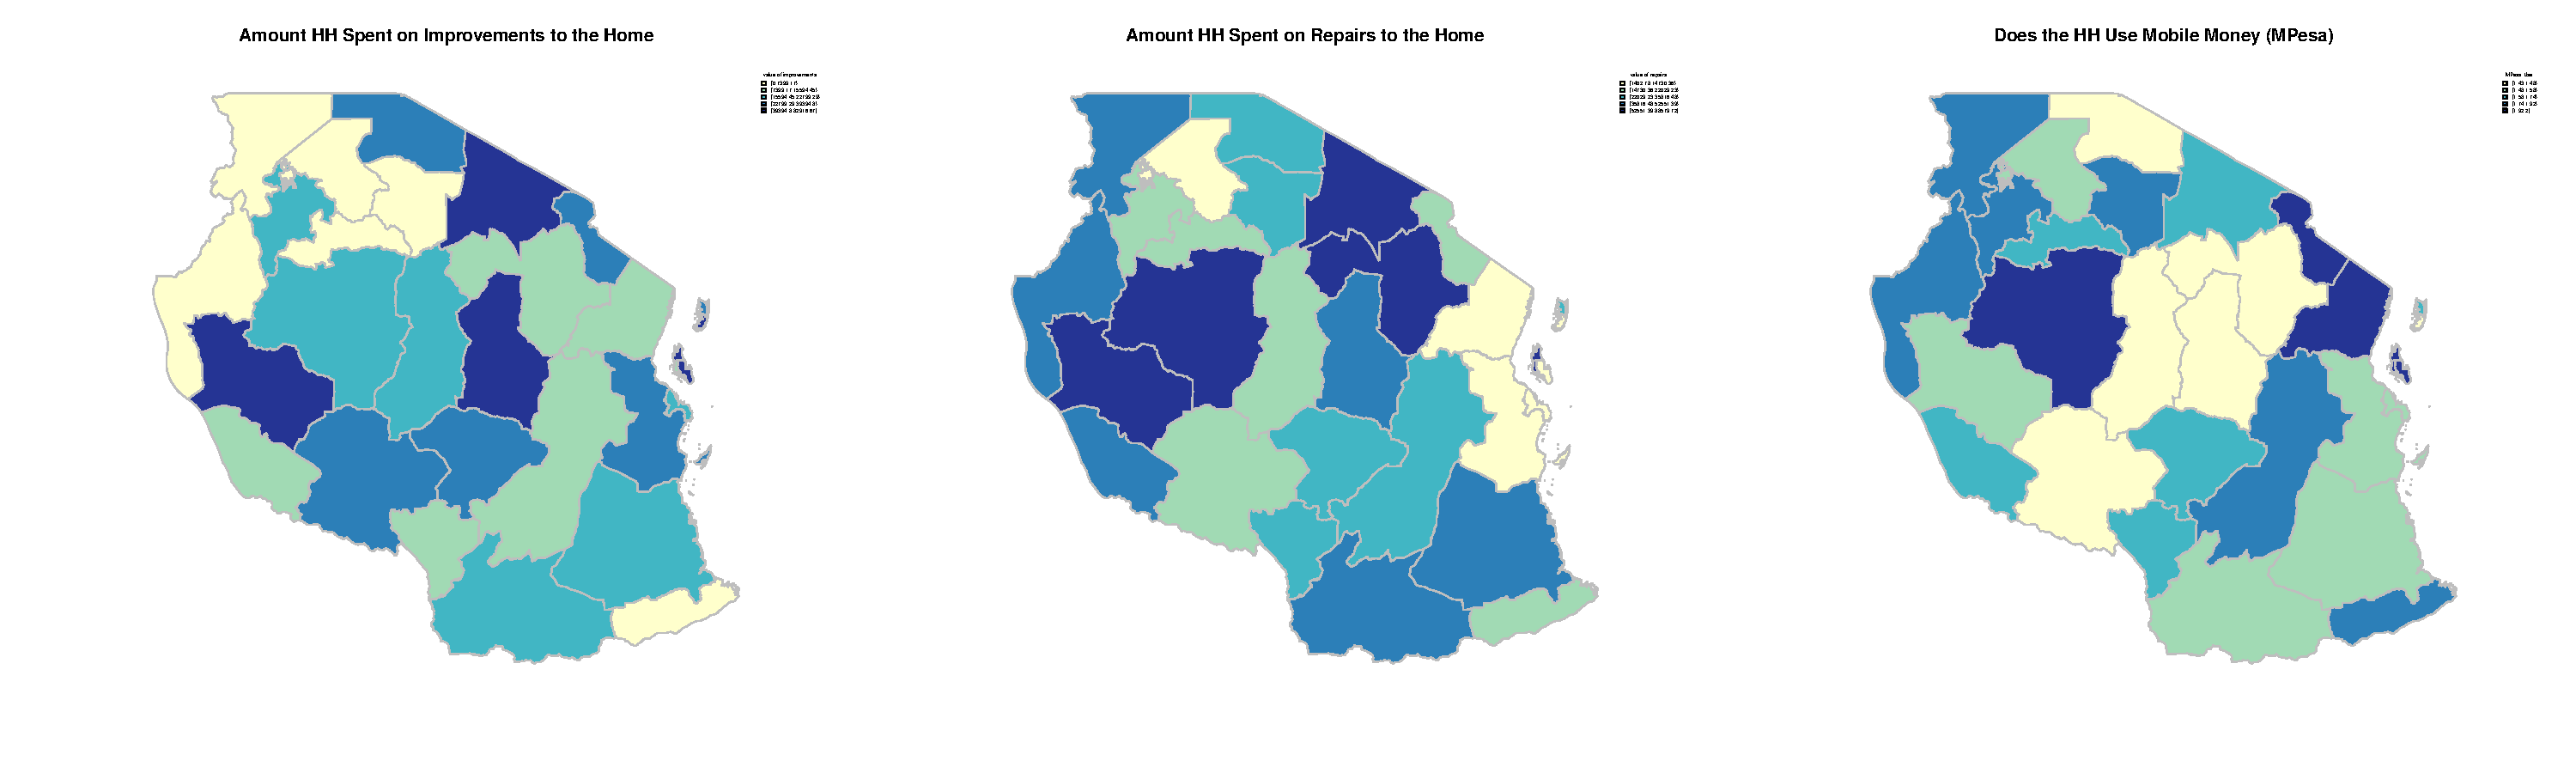
\includegraphics{PUBPOL599B_Final_Project_Exec-location}
\caption{Improvements to the Home, Repairs to the Home and Mobile Money Use by Region}
\end{figure}


  
\end{document}
